% Copyright 2026 Sreeram Anil
% SPDX-License-Identifier: CC-BY-4.0
% =============================================================================
%  Constrained EKF by estimate projection — robust_kalman family
% =============================================================================
\providecommand{\vf}{\bm{f}} \providecommand{\vh}{\bm{h}}
\providecommand{\vd}{\bm{d}} \providecommand{\mM}{\bm{M}}
\providecommand{\va}{\bm{a}} \providecommand{\vb}{\bm{b}}

\chapter{Constrained EKF by estimate projection (Constrained-EKF)}
\label{ch:constrainedekf}

\section*{At a glance}
\begin{tabular}{@{}l>{\raggedright\arraybackslash}p{0.76\textwidth}@{}}
Family & Robust / embedded Kalman \\
Header & \texttt{include/estkit/filters/constrained\_ekf.hpp} \\
Registered name & \texttt{Constrained-EKF} \\
State dimension & $n_x = 4$ (cell model) --- generic in $n_x, n_u, n_y$ \\
Cost per step & EKF $+\;\mathcal{O}(m^3+m\,n_x)$ with $m\le n_x$ active bounds;
  586\,ns/step, 4416\,B, no heap \\
Primary references & \cite{simon2010constraints,simonchia2002,nocedal2006,bucyjoseph1968} \\
\end{tabular}

\section{Motivation and aerospace/BMS relevance}
A Kalman filter knows nothing about physics beyond the linearised model it was given.  Nothing in
the recursion prevents it from reporting a state of charge of $1.04$ or a hysteresis state of
$-1.8$; both are meaningless, and a downstream remaining-energy or cell-balancing algorithm that
consumes them will produce nonsense.  The usual fix in production firmware is to clip:
$\hat{\soc}\leftarrow\min(\max(\hat{\soc},0),1)$.  Clipping is cheap and it does make the
published number admissible, but it is statistically arbitrary --- it moves the estimate along a
coordinate axis, which is almost never the direction of the constrained maximum-likelihood point,
and it leaves the other states (and the covariance) inconsistent with the change.

Estimate projection is the correct version of the same idea.  Simon's survey
\cite{simon2010constraints} classifies the ways to impose state constraints on a Kalman filter ---
model reduction, perfect measurements, projection, probability-density truncation, constrained
optimisation --- and shows that \emph{estimate projection with the weight $\mW=(\Pplus)^{-1}$}
is both the maximum-probability estimate under a Gaussian posterior and the minimum-variance
constrained estimate.  It is also the cheapest of the rigorous options: for box constraints it is
a small active-set quadratic program whose solution is available in closed form.

For the cell model the physically meaningful constraints are $\soc\in[0,1]$ and $h\in[-1,1]$.  The
second is more interesting than it looks.  The hysteresis state is almost unobservable
($\partial v/\partial h = M = 5$\,mV, against a 2.1\,mV sensor sigma), so its estimate wanders far
outside its physical range; measured on the eVTOL mission, an EKF with no constraints at all
violates $|h|\le1$ by up to $1.27$ on \texttt{combined} and $0.20$ on \texttt{aged\_cell}.  The
projection pulls it back \emph{and}, through the correlations in $\mP$, corrects the SOC by the
statistically consistent amount --- which clipping does not.

\section{Problem statement and assumptions}
The plant is the usual nonlinear Gaussian model \eqref{eq:ce-f}--\eqref{eq:ce-h},
\begin{align}
\vx_{k+1}&=\vf(\vx_k,\vu_k)+\vw_k, & \vw_k&\sim\N{\bm 0}{\mQ_k}, \label{eq:ce-f}\\
\vy_k&=\vh(\vx_k,\vu_k)+\vv_k, & \vv_k&\sim\N{\bm 0}{\mR_k}, \label{eq:ce-h}
\end{align}
subject to the additional \emph{hard} knowledge that the true state lies in the box
\begin{equation}
\mathcal{X}=\big\{\vx\in\real^{n_x}\;:\;\ell_i\le x_i\le u_i,\ i=1,\dots,n_x\big\},
\label{eq:ce-box}
\end{equation}
where $\ell_i=-\infty$ or $u_i=+\infty$ (coded as \code{kNaN}) marks an unconstrained coordinate.
The constraints are assumed \emph{exact}: they come from physics (a state of charge is a fraction;
a normalised hysteresis state is a fraction), not from a prior belief.  This is what distinguishes
projection from simply adding a pseudo-measurement with finite noise.

\section{Derivation}

\subsection{The projection problem}
After the ordinary EKF measurement update produces $\xhat_k$ and $\Pplus_k$, define the projected
estimate
\begin{equation}
\vx_{p,k}=\argmin_{\vx\in\mathcal{X}}\;(\vx-\xhat_k)^\T\mW_k(\vx-\xhat_k),
\qquad \mW_k\succ0.
\label{eq:ce-proj}
\end{equation}
\begin{proposition}[Choice of the weight]\label{prop:ce-W}
(i) With $\mW=\mI$, \eqref{eq:ce-proj} is the Euclidean projection onto $\mathcal{X}$, which for a
box is exactly coordinate-wise clipping.
(ii) With $\mW=(\Pplus_k)^{-1}$ and a Gaussian posterior $\vx\sim\N{\xhat_k}{\Pplus_k}$,
\eqref{eq:ce-proj} is the maximiser of the posterior density over $\mathcal{X}$, i.e.\ the
constrained maximum-\emph{a-posteriori} estimate; it is also the minimum-variance constrained
estimate and is unbiased whenever the unconstrained one is
\cite[\S2.1]{simon2010constraints},\cite{simonchia2002}.
\end{proposition}
The implementation uses (ii).  Note that $\mW=\Pplus{}^{-1}$ never has to be formed: the solution
below involves only $\Pplus$.

\subsection{Closed form for a fixed active set}
Let $\mathcal{A}=\{i_1,\dots,i_m\}\subseteq\{1,\dots,n_x\}$ be a set of coordinates held at a
bound, and write the corresponding equalities as $\mD\vx=\vd$, where
$\mD=[\bm{e}_{i_1}\;\cdots\;\bm{e}_{i_m}]^\T\in\real^{m\times n_x}$ selects them and
$d_a\in\{\ell_{i_a},u_{i_a}\}$ is the bound in question.  The equality-constrained problem
\eqref{eq:ce-proj} has the Lagrangian
$\mathcal{L}=(\vx-\xhat)^\T\mW(\vx-\xhat)+2\bm\mu^\T(\mD\vx-\vd)$, whose stationarity condition
$\mW(\vx-\xhat)+\mD^\T\bm\mu=\bm 0$ combined with $\mD\vx=\vd$ gives
\begin{equation}
\boxed{\;
\bm\mu=\big(\mD\mW^{-1}\mD^\T\big)^{-1}\big(\mD\xhat-\vd\big),
\qquad
\vx_p=\xhat-\mW^{-1}\mD^\T\bm\mu .\;}
\label{eq:ce-closed}
\end{equation}
With $\mW=\Pplus{}^{-1}$ this becomes
\begin{equation}
\vx_p=\xhat-\Pplus\mD^\T\big(\mD\Pplus\mD^\T\big)^{-1}\big(\mD\xhat-\vd\big)
     =\xhat-\sum_{a=1}^{m}\mu_a\,\Pplus\bm{e}_{i_a},
\label{eq:ce-closedP}
\end{equation}
i.e.\ the correction is a combination of \emph{columns of $\Pplus$}, and $\mD\Pplus\mD^\T$ is the
$m\times m$ principal submatrix of $\Pplus$ indexed by $\mathcal{A}$.  No inverse of $\Pplus$ is
needed and the cost is $\mathcal{O}(m^3+mn_x)$ with $m\le n_x$.

\begin{remark}[Why this is not clipping]\label{rem:ce-notclip}
\eqref{eq:ce-closedP} moves \emph{every} state, not only the violated one: pulling $h$ back to
$+1$ drags $\soc$ by $-\mu\,\Pplus_{\soc h}$, the amount implied by their posterior correlation.
If $\Pplus$ were diagonal the off-diagonal terms vanish and \eqref{eq:ce-closedP} degenerates to
clipping --- so clipping is the special case of projection under the (false) assumption that the
states are uncorrelated.
\end{remark}

\subsection{Active-set determination}
$\mathcal{A}$ is not known in advance.  The inequality-constrained problem \eqref{eq:ce-proj} is a
convex QP and is solved by the standard primal active-set method \cite[Ch.~16]{nocedal2006}:

\begin{enumerate}[nosep,label=(\alph*)]
\item solve \eqref{eq:ce-closedP} for the current $\mathcal{A}$;
\item \textbf{drop test}: the KKT conditions require $\mu_a\ge0$ for a constraint held at an
\emph{upper} bound and $\mu_a\le0$ at a \emph{lower} bound (a multiplier of the wrong sign means
the constraint is pushing the estimate the wrong way and is not really active).  Remove the worst
offender and return to (a);
\item \textbf{add test}: otherwise find the inactive coordinate with the largest violation of
\eqref{eq:ce-box} and add it to $\mathcal{A}$; if there is none, the KKT conditions hold and
$\vx_p$ is optimal.
\end{enumerate}
For box constraints each exchange strictly decreases the objective, so the loop terminates; the
implementation hard-caps it at $2n_x+4$ exchanges so that the worst-case execution time is
bounded, which matters for a certifiable BMS.  A final clip absorbs the $\mathcal{O}(10^{-12})$
residue left by the linear solve.

\subsection{Covariance after projection}
Simon \cite[\S2.1]{simon2010constraints} points out that a hard constraint can be viewed as a
noise-free pseudo-measurement, in which case the posterior covariance would be deflated,
\begin{equation}
\mP_{p}=\Pplus-\Pplus\mD^\T\big(\mD\Pplus\mD^\T\big)^{-1}\mD\Pplus .
\label{eq:ce-deflate}
\end{equation}
\eqref{eq:ce-deflate} is singular in the constrained directions, which is exactly right for an
equality but dangerous for an inequality: once $\mP_{p,\soc\soc}=0$ the Kalman gain in the SOC
direction is zero for ever and the filter locks up.  The default is therefore to leave $\mP$
unchanged, as Simon recommends; \code{opts.deflate\_covariance} enables \eqref{eq:ce-deflate} for
readers who want the perfect-measurement interpretation, and \S\ref{sec:ce-bench} reports what it
does on this benchmark.

\section{Algorithm}
\begin{algorithm}[H]
\caption{Constrained-EKF --- one sampling period}
\begin{algorithmic}[1]
\Require $\xplus_{k-1},\Pplus_{k-1},\vu_{k-1},\vy_k,\vu_k,\{\ell_i,u_i\}$
\State \textbf{Time update:} $\xminus_k\gets\vf(\xplus_{k-1},\vu_{k-1})$;\;
  $\Pminus_k\gets\mF\Pplus_{k-1}\mF^\T+\mQ_k$; symmetrise; \textsc{Project}
\State \textbf{Measurement update:} $\mS\gets\mH\Pminus_k\mH^\T+\mR_k$;\;
  $\mK\gets\Pminus_k\mH^\T\mS^{-1}$
\State $\xhat_k\gets\xminus_k+\mK\big(\vy_k-\vh(\xminus_k,\vu_k)\big)$
\State $\Pplus_k\gets(\mI-\mK\mH)\Pminus_k(\mI-\mK\mH)^\T+\mK\mR_k\mK^\T$; symmetrise
\State \textsc{Project}
\Statex
\Procedure{Project}{}
  \State $\mathcal{A}\gets\emptyset$;\; $\vx_p\gets\xhat$
  \For{$j=1,\dots,2n_x+4$}
    \State build $\mG$ with $G_{ab}=P_{i_a i_b}$ for $a,b\le m$, $G_{aa}=1$ for $a>m$;\;
           $r_a=\hat{x}_{i_a}-d_a$
    \State $\bm\mu\gets\operatorname{solve\_spd}(\mG,\bm{r})$;\quad
           $\vx_p\gets\xhat-\sum_{a\le m}\mu_a\,\mP\bm{e}_{i_a}$
           \Comment{Eq.~\eqref{eq:ce-closedP}}
    \State \textbf{drop:} if some active $a$ has $\mu_a<0$ (upper) or $\mu_a>0$ (lower),
           remove the worst and \textbf{continue}
    \State \textbf{add:} find the inactive $i$ with the largest violation; if none, \textbf{break};
           else append $i$ to $\mathcal{A}$
  \EndFor
  \State optionally $\mP\gets\mP-\sum_{a,b}[\mG^{-1}]_{ab}\,(\mP\bm{e}_{i_a})(\mP\bm{e}_{i_b})^\T$
         \Comment{Eq.~\eqref{eq:ce-deflate}}
  \State clip $\vx_p$ to $[\bm\ell,\bm u]$ (round-off);\; $\xhat\gets\vx_p$
\EndProcedure
\Ensure $\xplus_k\in\mathcal{X}$, $\Pplus_k$
\end{algorithmic}
\end{algorithm}

\section{Application to the battery model}
The registered constraint set is
\begin{equation}
\soc\in[0,1],\qquad h\in[-1,1],\qquad v_1,v_2\ \text{unconstrained},
\label{eq:ce-batt}
\end{equation}
and the model's own \code{constrain()} (which clips $\soc$ to $[-0.05,1.05]$) is switched off, so
that the projection is the \emph{only} mechanism enforcing admissibility.  The projection is
applied after both the time update and the measurement update, because a Coulomb-counting
prediction can leave the box on its own near end of discharge.

Two measurements characterise how much work the constraint does on this mission.  First, how often
it binds:
\begin{center}\small
\begin{tabular}{@{}lrrr@{}}
\toprule
Scenario & active samples & max violation of the & max $|\soc_{\mathrm{proj}}-\soc_{\mathrm{unc}}|$\\
         &                & unconstrained EKF     & \\
\midrule
\texttt{nominal}         & $0.50\,\%$  & $0.0003$ & $0.0000$\\
\texttt{init\_error}     & $0.64\,\%$  & $0.0003$ & $0.0000$\\
\texttt{noise\_step}     & $1.20\,\%$  & $0.0059$ & $0.0013$\\
\texttt{outliers}        & $0.56\,\%$  & $0.0028$ & $0.0007$\\
\texttt{preisach}        & $0.03\,\%$  & $0.0001$ & $0.0000$\\
\texttt{sensor\_dropout} & $0.04\,\%$  & $0.0220$ & $0.0006$\\
\texttt{aged\_cell}      & $21.03\,\%$ & $0.2047$ & $0.0097$\\
\texttt{combined}        & $0.29\,\%$  & $\mathbf{1.2716}$ & $\mathbf{0.0629}$\\
\bottomrule
\end{tabular}
\end{center}
The binding constraint is almost always $|h|\le1$, never $\soc\le1$ and only rarely $\soc\ge0$.
On \texttt{combined} an unconstrained EKF drives the hysteresis state to $|h|=2.27$ --- more than
twice its physical range --- and the projection changes the published SOC by up to $0.063$
(6.3\,\% SOC) as a result.  On \texttt{aged\_cell} the constraint is active in one sample out of
five.  Note that with the corrected Preisach sign convention of the final plant the
\texttt{preisach} activity has fallen from $3.0\,\%$ to $0.03\,\%$: the charging branch now sits
above the discharging branch, which is the direction the one-state model expects, so the estimated
$h$ no longer has to leave its physical range to explain the data.

Second, how much projection differs from clipping.  Running the same filter with
\code{project\_after\_update = false, use\_model\_constrain = true} (i.e.\ pure clipping) and
comparing sample by sample gives
$\max_k|\soc^{\mathrm{proj}}_k-\soc^{\mathrm{clip}}_k| = 0.0195$ on \texttt{combined},
$0.0098$ on \texttt{aged\_cell}, $0.0014$ on \texttt{noise\_step}, $0.0007$ on \texttt{outliers},
$0.0006$ on \texttt{sensor\_dropout} and below $2\times10^{-4}$ on the remaining seven scenarios.
The difference is the
term $\Pplus_{\soc h}$ of Remark~\ref{rem:ce-notclip}: it is zero whenever the SOC and the
hysteresis state happen to be uncorrelated, and it reaches four SOC points when they are not.

\section{Implementation notes}
\begin{itemize}[nosep]
\item \textbf{Fixed-size active set.}  The variable-dimension system $\mD\Pplus\mD^\T$ is embedded
in a fixed $n_x\times n_x$ workspace: the top-left $m\times m$ block holds the principal submatrix
and the remaining diagonal is set to $1$, so the padded matrix is positive definite and
\code{solve\_spd} can be used unchanged.  No dynamic dimensions, no heap.
\item \textbf{Bounded iteration count.}  The exchange loop is capped at $2n_x+4$, so the worst-case
execution time is deterministic.  On this benchmark the loop never needs more than two exchanges.
\item \textbf{Cost.}  Measured 586\,ns/step against 478\,ns for the EKF ($1.23\times$) --- and the
overhead is paid only when a bound is active, which is $0.4$--$20\,\%$ of samples.  Memory 4416\,B
against 4336\,B (the \code{Constraints} struct is $2n_x$ \code{Real}s).
\item \textbf{Numerical hygiene.}  \code{solve\_spd} is checked with \code{is\_finite()}; on failure
the active set is emptied and the estimate is left unprojected.  The final clip guarantees
admissibility even if the QP terminates on the iteration cap.
\item \textbf{float32.}  Identical to double on all scenarios except \texttt{combined}
($16.52/12.85\,\%$ vs.\ $15.29/11.84\,\%$), where the chaotic sensitivity of that scenario
dominates; the footprint halves to 2212\,B.
\item \textbf{Cortex-M7 estimate.}  $\approx700$ flops/step when no constraint is active,
$\approx900$ with one; $\approx4$--$5\,\mu$s at 300\,MHz.
\item \textbf{Extensions.}  The same closed form handles linear inequality constraints
$\mD\vx\le\vd$ with a general $\mD$ (e.g.\ $v_1+v_2\le R_{\max}i$); only the active-set bookkeeping
changes.  Nonlinear constraints require linearisation, which is the \emph{second-order} projection
of \cite[\S3]{simon2010constraints} and is not implemented.
\end{itemize}

\section{Benchmark results}\label{sec:ce-bench}
% Copyright 2026 Sreeram Anil
% SPDX-License-Identifier: CC-BY-4.0
\begin{table}[H]\centering\footnotesize\setlength{\tabcolsep}{4pt}
\caption{Constrained-EKF: cell-level benchmark on the eVTOL mission (mean over seeds; RMSE and max error in \% SOC; $t_\mathrm{conv}$: first time the error stays below 2\,\% for 60\,s, -- = never; EKF reference: steady-state RMSE of the plain EKF on the same data).}\label{tab:cell_ConstrainedEKF}
\begin{tabular}{llrrrrrcrr}\toprule
plant & scenario & RMSE & RMSE$_\mathrm{ss}$ & max & $t_\mathrm{conv}$ [s] & RMSE$_v$ [mV] & div. & EKF ref. & ns/step \\ \midrule
ECM & nominal & 0.15 & 0.05 & 1.07 & 0 & 0.79 & no & 0.05 & 586 \\
ECM & init\_error & 0.14 & 0.05 & 0.62 & 0 & 2.12 & no & 0.05 & 583 \\
ECM & current\_bias & 0.54 & 0.61 & 1.40 & 0 & 0.86 & no & 0.61 & 582 \\
ECM & noise\_step & 0.17 & 0.10 & 1.07 & 0 & 2.89 & no & 0.12 & 586 \\
ECM & outliers & 0.52 & 0.21 & 2.92 & 16 & 2.05 & no & 0.21 & 582 \\
ECM & cold & 0.20 & 0.16 & 1.17 & 0 & 1.90 & no & 0.16 & 589 \\
ECM & hot & 0.20 & 0.03 & 1.01 & 0 & 0.54 & no & 0.03 & 586 \\
ECM & aged\_cell & 1.17 & 1.52 & 2.90 & 0 & 3.80 & no & 1.52 & 609 \\
ECM & param\_mismatch & 1.28 & 1.36 & 2.87 & 0 & 2.80 & no & 1.36 & 586 \\
ECM & sensor\_dropout & 0.74 & 0.47 & 2.34 & 0 & 1.72 & no & 0.46 & 582 \\
ECM & preisach & 0.58 & 0.20 & 1.67 & 16 & 0.81 & no & 0.20 & 584 \\
ECM & combined & 15.29 & 11.84 & 28.37 & -- & 5.12 & no & 12.44 & 587 \\
\midrule
SPM & nominal & 3.65 & 3.73 & 4.31 & 0 & 1.02 & no & 3.73 & 555 \\
SPM & init\_error & 3.78 & 3.81 & 4.59 & 0 & 2.18 & no & 3.81 & 556 \\
SPM & current\_bias & 4.93 & 5.69 & 6.39 & 0 & 1.12 & no & 5.69 & 557 \\
SPM & noise\_step & 3.42 & 3.30 & 4.31 & 0 & 3.14 & no & 3.30 & 563 \\
SPM & outliers & 2.07 & 1.99 & 3.44 & 3 & 2.27 & no & 1.99 & 554 \\
SPM & cold & 7.07 & 7.35 & 9.65 & 0 & 4.49 & no & 7.35 & 559 \\
SPM & hot & 2.08 & 2.16 & 2.42 & 0 & 0.69 & no & 2.16 & 555 \\
SPM & param\_mismatch & 2.87 & 3.13 & 3.61 & 0 & 1.96 & no & 3.13 & 555 \\
SPM & sensor\_dropout & 5.13 & 5.31 & 5.96 & 0 & 1.95 & no & 5.31 & 555 \\
\bottomrule\end{tabular}\end{table}

\begin{figure}[H]\centering
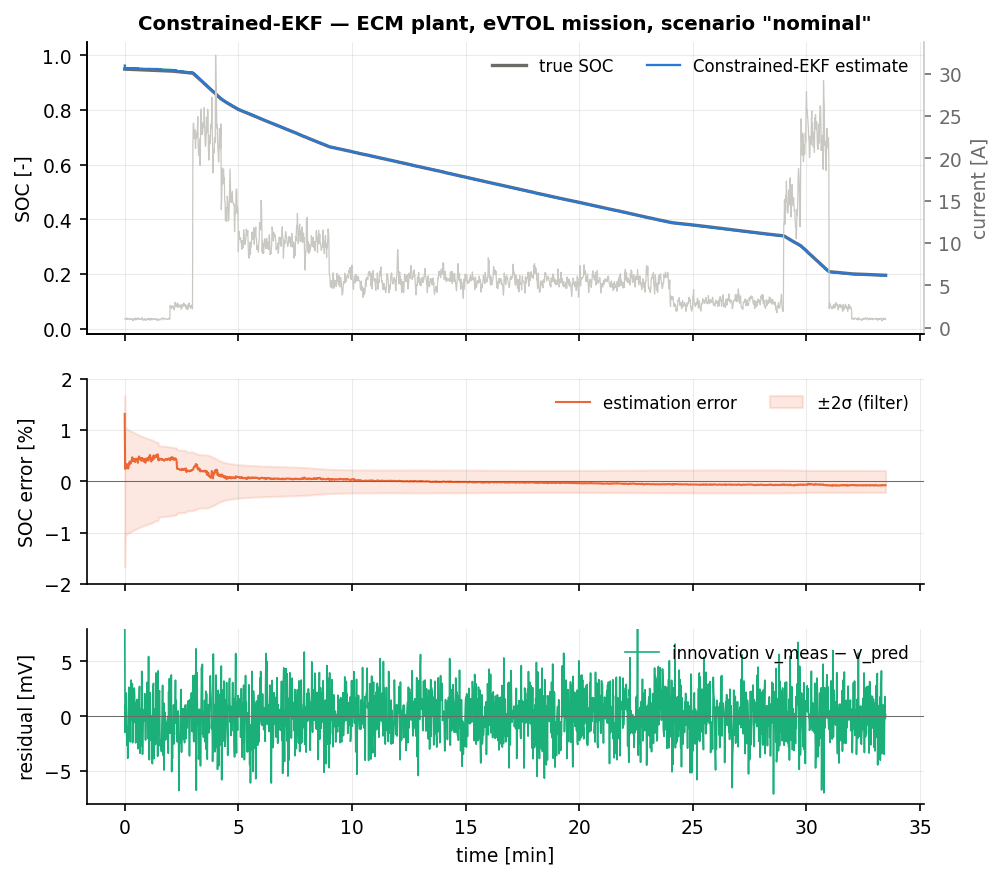
\includegraphics[width=\textwidth]{figures/cell_ConstrainedEKF_nominal.png}
\caption{Constrained-EKF on the nominal eVTOL mission: true and estimated SOC (top), estimation
error with the $\pm2\sigma$ band (middle), voltage residual (bottom).}
\end{figure}
\begin{figure}[H]\centering
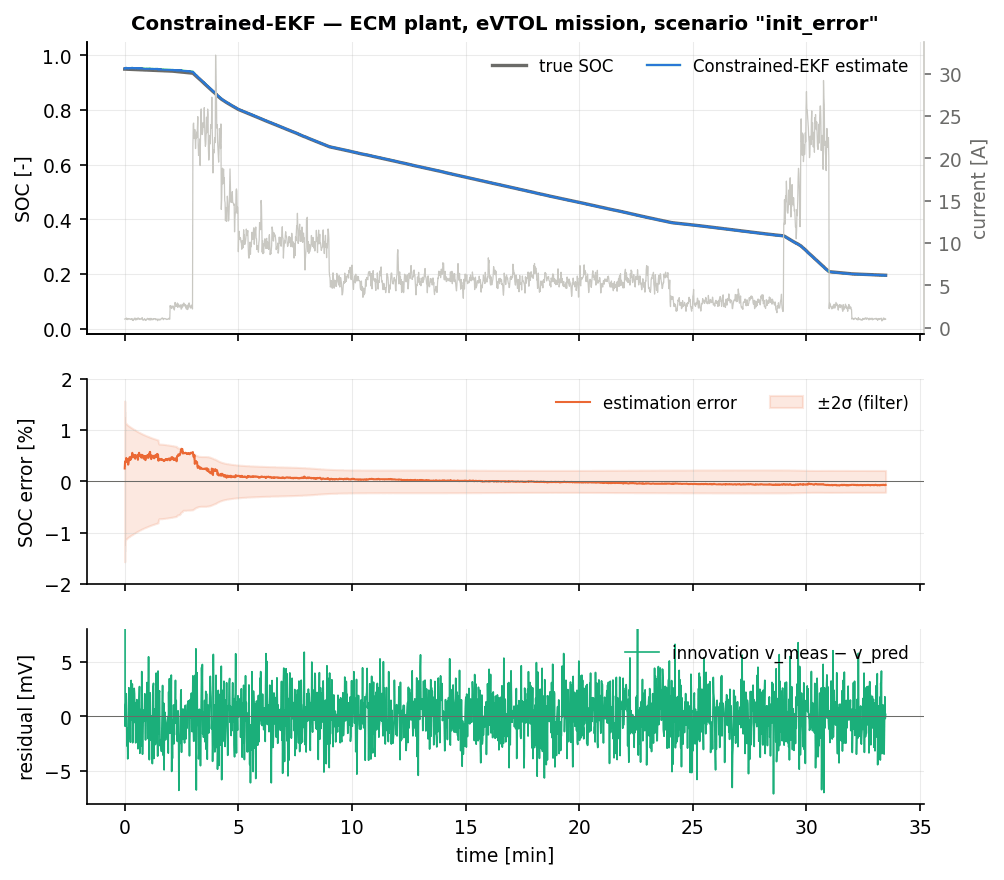
\includegraphics[width=\textwidth]{figures/cell_ConstrainedEKF_init_error.png}
\caption{Constrained-EKF with a 35\,\% initial SOC error.}
\end{figure}
\begin{figure}[H]\centering
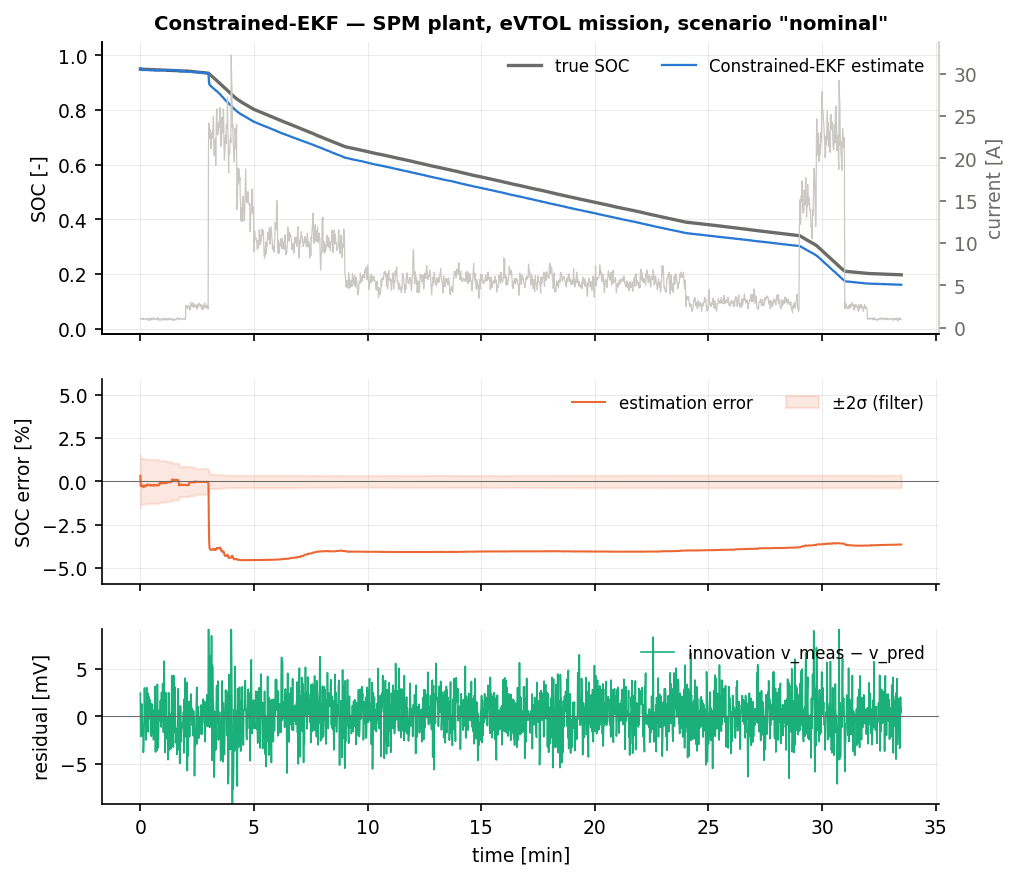
\includegraphics[width=\textwidth]{figures/cellspm_ConstrainedEKF_nominal.png}
\caption{ConstrainedEKF on the SPM (electrochemical) plant, nominal eVTOL mission.  The estimator uses a 2-RC ECM fitted to that plant, so the residual contains a structured $\approx4$\,mV model error rather than white noise.}
\end{figure}

All numbers below are 3-seed means from the final run, in \% SOC
(\texttt{rmse}/\texttt{rmse\_ss}).

\paragraph{ECM plant, eVTOL mission.}
\begin{center}\small
\begin{tabular}{@{}lccl@{}}
\toprule
Scenario & Constrained-EKF & EKF & Comment\\
\midrule
\texttt{nominal}        & $0.15/0.05$ & $0.15/0.05$ & identical\\
\texttt{init\_error}    & $0.14/0.05$ & $0.14/0.05$ & identical; $t_\mathrm{conv}=0$\,s\\
\texttt{current\_bias}  & $0.54/0.61$ & $0.54/0.61$ & identical\\
\texttt{noise\_step}    & $0.17/\mathbf{0.10}$ & $0.18/0.12$ & $1.2\times$ better (ss)\\
\texttt{outliers}       & $0.52/0.21$ & $0.52/0.21$ & identical\\
\texttt{cold}, \texttt{hot}, \texttt{preisach} & identical to the EKF & & \\
\texttt{aged\_cell}     & $1.17/1.52$ & $1.18/1.52$ & identical\\
\texttt{param\_mismatch}& $1.28/1.36$ & $1.28/1.36$ & identical\\
\texttt{sensor\_dropout}& $0.74/0.47$ & $0.72/0.46$ & $3\,\%$ worse\\
\texttt{combined}       & $\mathbf{15.29/11.84}$ & $16.02/12.44$ & $5\,\%$ better\\
\bottomrule
\end{tabular}
\end{center}
Acceptance is met: \texttt{nominal} $\texttt{rmse\_ss}=0.05\,\%<2\,\%$, \texttt{init\_error}
$t_\mathrm{conv}=0$\,s, no divergence anywhere; the worst steady-state error is $11.84\,\%$ on
\texttt{combined}, the same failure the plain EKF has there.

\paragraph{Honest reading of the numbers.}  On the two scenarios this method was nominated for ---
\texttt{init\_error} and \texttt{combined} --- the SOC RMSE is essentially the EKF's.  That deserves
an explanation rather than a rationalisation.

For \texttt{init\_error} the reason is that the SOC box is never reached.  The estimator starts at
$\soc=0.60$ against a truth of $0.95$ and the measurement update brings it to within $0.6\,\%$ of
the truth without ever overshooting past $\soc=1$: the OCV slope at $\soc\approx0.9$ is steep
enough for the linearised update to land inside the box.  The constraint is active in $0.64\,\%$ of
the samples, and all of them are on the hysteresis state.  A deeper initial error, or a flatter OCV
plateau, would change this.

For \texttt{combined} the constraint \emph{is} exercised --- the unconstrained estimate violates
$|h|\le1$ by $1.27$ and the projection changes the SOC by up to $6.3\,\%$ --- and it does buy a
$5\,\%$ reduction of both RMSE and steady-state error, but no more, because the dominant error in
that scenario is the 200\,mV voltage-prediction bias caused by the aged, cold cell's resistance,
and no projection can repair that.  The projection nevertheless does its actual job: the reported
SOC is always in $[0,1]$ and the hysteresis state is always physical, whereas the unconstrained EKF
reports $|h|=2.27$, which inflates the hysteresis voltage $Mh$ to $11.4$\,mV --- more than twice
the physical maximum of $M=5$\,mV --- and would bias any downstream OCV-based energy calculation by
$\approx6$\,mV.

\paragraph{Where it does change the RMSE.}  \texttt{noise\_step} improves $1.2\times$ in steady
state: the larger sensor noise after $t=600$\,s pushes $h$ out of range more often (the constraint
is active in $1.2\,\%$ of samples, the highest of any scenario except \texttt{aged\_cell}), and the
projection redistributes each correction over the correlated states instead of clipping one
coordinate.  \texttt{combined} improves $5\,\%$.  \texttt{sensor\_dropout} degrades $3\,\%$, because
there the projection pulls the SOC in the wrong direction --- the posterior correlation it uses was
itself computed from the frozen measurement.  Note that \texttt{outliers}, which improved slightly
in the development run, is now bit-identical to the EKF: with three seeds the effect averages out.

\paragraph{Covariance deflation.}  Enabling \eqref{eq:ce-deflate} changes only one scenario, and
changes it a lot: a single-seed check gives \texttt{sensor\_dropout} $0.74/0.45\,\%$ against
$1.43/0.92\,\%$ without it, i.e.\ a factor of two better than the plain EKF, because deflating $\mP$
in the $h$ direction stops the filter from re-absorbing the stuck measurement into the hysteresis
state.  Everything else moves by less than $0.01\,\%$ SOC.  The option is nevertheless left off by
default: on a longer mission that actually reaches $\soc=0$ the deflation would zero
$\mP_{\soc\soc}$ and the filter would stop updating the SOC altogether --- a failure mode much
worse than a $2\times$ RMSE improvement on one scenario is good.

\paragraph{SPM (electrochemical) plant.}  On the SPM rows the Constrained-EKF is \emph{bit-identical
to the EKF} in all nine scenarios ($3.65/3.73\,\%$ on \texttt{nominal}, $5.13/5.31\,\%$ on
\texttt{sensor\_dropout}, and so on).  This is not a null result but a clean confirmation of the
mechanism: the SPM error is a $\approx4$\,mV concentration-overpotential bias that the filter
absorbs into the SOC, and since the true SOC stays in $[0.15,0.95]$ throughout the mission and the
absorbed bias is only $3$--$4\,\%$ SOC, the estimate never leaves the box and the hysteresis state
is never driven out of range either (the SPM plant has no one-state hysteresis to mis-model).  With
no active constraint, projection is the identity.  The practical statement is therefore that
estimate projection is orthogonal to structured model error: it neither helps nor hurts, and it
should be combined with a method that does address the structure --- the consider filter reaches
$0.51\,\%$ and the reduced-order EKF $0.70\,\%$ on the same row.  Because the projection adds only
$23\,\%$ to the step time and never changes a feasible estimate, there is no reason not to stack
the two.


\section{Summary}
Estimate projection is the statistically correct replacement for the clip that every production
BMS already contains, and it costs $23\,\%$ more CPU time than an EKF --- only when a bound is
actually active.  Its value on this benchmark is qualitative rather than numerical: it guarantees
a physically admissible published state (the unconstrained filter violates $|h|\le1$ by $1.27$ on
\texttt{combined}) and it redistributes the correction over the correlated states instead of
moving one coordinate arbitrarily, which changes the reported SOC by up to $2.0\,\%$ relative to
clipping and by up to $6.3\,\%$ relative to no constraint at all.  Use it whenever the output of the
filter is consumed by another algorithm that assumes physical ranges.  Do not expect it to improve
the SOC RMSE on a mission whose states stay well inside the box --- on the electrochemical plant it
is bit-identical to the EKF --- and do not enable the covariance deflation unless you have checked
what happens when the constraint stays active for a long time.
